\documentclass{article}
\usepackage[margin=1in]{geometry}
\usepackage{amsmath,amsthm,amssymb}
\usepackage{bbm,enumerate,mathtools}
\usepackage{tikz,pgfplots}
\usepackage{chessboard}
\usepackage[hidelinks]{hyperref}
\usepackage{multicol} % Problem 35

\newenvironment{question}{\begin{trivlist}\item[\textbf{Question.}]}{\end{trivlist}}
\newenvironment{note}{\begin{trivlist}\item[\textbf{Note.}]}{\end{trivlist}}
\newenvironment{references}{\begin{trivlist}\item[\textbf{References.}]}{\end{trivlist}}
\newenvironment{related}{\begin{trivlist}\item[\textbf{Related.}]\end{trivlist}\begin{enumerate}}{\end{enumerate}}


\begin{document}
\rating{3}{3}
Consider polyominoes where each cell has one of $n$ colors, and
each distinct pair of colors is adjacent (horizontally or vertically) to each other
somewhere in the polyomino. Let an $n$-minimum polyomino be one that has the
minimum number of cells.

\begin{figure}[!h]
  \centering
  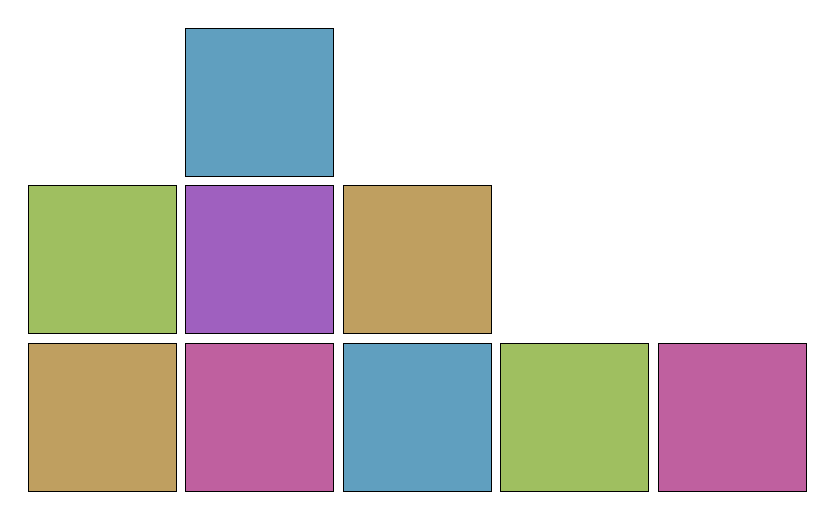
\begin{tikzpicture}[scale=2]
    \def\polyomino{
      1/3/0/2/3,
      0/2/2/3/0,
      1/2/2/0/3,
      2/2/3/2/0,
      0/1/3/2/0,
      1/1/3/0/2,
      2/1/0/2/3,
      3/1/2/3/0,
      4/1/3/0/2
    }

    \foreach \x/\y/\r/\g/\b in \polyomino {
      \draw[fill={rgb:red,\r;green,\g;blue,\b;white,3}] (\x - 0.47, \y - 0.47) rectangle (\x + 0.47, \y + 0.47);
    }
  \end{tikzpicture}
  \caption{An example of a minimum polyomino for $n = 5$; $a(5)=9$}
\end{figure}

\begin{question}
  How many such $n$-minimum polyominoes exist?
\end{question}
\begin{related}
  \item What if the ``distinct'' restriction is lifted?
    (e.g. a blue label must somewhere be adjacent to another blue label.)
  \item What is a way to determine the size of an $n$-minimum polyomino for
    large $n$?
  \item What if this is done on a triangular or hexagonal grid?
  \item What if this is done on a three dimensional cube lattice?
\end{related}

\begin{references}
  \item \url{https://oeis.org/A278299}
  \item \url{http://www.peterkagey.com/square_games}
\end{references}
\end{document}
